\documentclass[11pt]{article}
\renewcommand{\arraystretch}{1.5} % Default value: 1
\usepackage{sectsty}
\allsectionsfont{\color{blue}\fontfamily{lmss}\selectfont}
\usepackage{fontspec}
\setmainfont{XCharter}

\usepackage{listings}
\lstset{
basicstyle=\small\ttfamily,
tabsize=8,
columns=flexible,
breaklines=true,
frame=tb,
rulecolor=\color[rgb]{0.8,0.8,0.7},
backgroundcolor=\color[rgb]{1,1,0.91},
postbreak=\raisebox{0ex}[0ex][0ex]{\ensuremath{\color{red}\hookrightarrow\space}}
}
\usepackage{fontawesome}


\usepackage{mdframed}
\newmdenv[
  backgroundcolor=gray,
  fontcolor=white,
  nobreak=true,
]{terminalinput}



\usepackage{parskip}




    \usepackage[T1]{fontenc}
    % Nicer default font than Computer Modern for most use cases
    \usepackage{palatino}

    % Basic figure setup, for now with no caption control since it's done
    % automatically by Pandoc (which extracts ![](path) syntax from Markdown).
    \usepackage{graphicx}
    % We will generate all images so they have a width \maxwidth. This means
    % that they will get their normal width if they fit onto the page, but
    % are scaled down if they would overflow the margins.
    \makeatletter
    \def\maxwidth{\ifdim\Gin@nat@width>\linewidth\linewidth
    \else\Gin@nat@width\fi}
    \makeatother
    \let\Oldincludegraphics\includegraphics
    % Set max figure width to be 80% of text width, for now hardcoded.
\renewcommand{\includegraphics}[1]{\Oldincludegraphics[width=.8\maxwidth, height=.55\textheight, keepaspectratio]{#1}}
    % Ensure that by default, figures have no caption (until we provide a
    % proper Figure object with a Caption API and a way to capture that
    % in the conversion process - todo).
    \usepackage{caption}
    \DeclareCaptionLabelFormat{nolabel}{}
    \captionsetup{labelformat=nolabel, textfont=bf}

    \usepackage{adjustbox} % Used to constrain images to a maximum size
    \usepackage{xcolor} % Allow colors to be defined
    \usepackage{enumerate} % Needed for markdown enumerations to work
    \usepackage{geometry} % Used to adjust the document margins
    \usepackage{amsmath} % Equations
    \usepackage{amssymb} % Equations
    \usepackage{textcomp} % defines textquotesingle
    % Hack from http://tex.stackexchange.com/a/47451/13684:
    \AtBeginDocument{%
        \def\PYZsq{\textquotesingle}% Upright quotes in Pygmentized code
    }
    \usepackage{upquote} % Upright quotes for verbatim code
    \usepackage{eurosym} % defines \euro
    \usepackage[mathletters]{ucs} % Extended unicode (utf-8) support
    \usepackage[utf8x]{inputenc} % Allow utf-8 characters in the tex document
    \usepackage{fancyvrb} % verbatim replacement that allows latex
    \usepackage{grffile} % extends the file name processing of package graphics
                         % to support a larger range
    % The hyperref package gives us a pdf with properly built
    % internal navigation ('pdf bookmarks' for the table of contents,
    % internal cross-reference links, web links for URLs, etc.)
    \usepackage{hyperref}
    \usepackage{longtable} % longtable support required by pandoc >1.10
    \usepackage{booktabs}  % table support for pandoc > 1.12.2
    \usepackage[normalem]{ulem} % ulem is needed to support strikethroughs (\sout)
                                % normalem makes italics be italics, not underlines
    \usepackage{float}



    % Colors for the hyperref package
    \definecolor{urlcolor}{rgb}{0,.145,.698}
    \definecolor{linkcolor}{rgb}{.71,0.21,0.01}
    \definecolor{citecolor}{rgb}{.12,.54,.11}

    % ANSI colors
    \definecolor{ansi-black}{HTML}{3E424D}
    \definecolor{ansi-black-intense}{HTML}{282C36}
    \definecolor{ansi-red}{HTML}{E75C58}
    \definecolor{ansi-red-intense}{HTML}{B22B31}
    \definecolor{ansi-green}{HTML}{00A250}
    \definecolor{ansi-green-intense}{HTML}{007427}
    \definecolor{ansi-yellow}{HTML}{DDB62B}
    \definecolor{ansi-yellow-intense}{HTML}{B27D12}
    \definecolor{ansi-blue}{HTML}{208FFB}
    \definecolor{ansi-blue-intense}{HTML}{0065CA}
    \definecolor{ansi-magenta}{HTML}{D160C4}
    \definecolor{ansi-magenta-intense}{HTML}{A03196}
    \definecolor{ansi-cyan}{HTML}{60C6C8}
    \definecolor{ansi-cyan-intense}{HTML}{258F8F}
    \definecolor{ansi-white}{HTML}{C5C1B4}
    \definecolor{ansi-white-intense}{HTML}{A1A6B2}

    % commands and environments needed by pandoc snippets
    % extracted from the output of `pandoc -s`
    \providecommand{\tightlist}{%
      \setlength{\itemsep}{0pt}\setlength{\parskip}{0pt}}
    \DefineVerbatimEnvironment{Highlighting}{Verbatim}{commandchars=\\\{\}}
    % Add ',fontsize=\small' for more characters per line
    \newenvironment{Shaded}{}{}
    \newcommand{\KeywordTok}[1]{\textcolor[rgb]{0.00,0.44,0.13}{\textbf{{#1}}}}
    \newcommand{\DataTypeTok}[1]{\textcolor[rgb]{0.56,0.13,0.00}{{#1}}}
    \newcommand{\DecValTok}[1]{\textcolor[rgb]{0.25,0.63,0.44}{{#1}}}
    \newcommand{\BaseNTok}[1]{\textcolor[rgb]{0.25,0.63,0.44}{{#1}}}
    \newcommand{\FloatTok}[1]{\textcolor[rgb]{0.25,0.63,0.44}{{#1}}}
    \newcommand{\CharTok}[1]{\textcolor[rgb]{0.25,0.44,0.63}{{#1}}}
    \newcommand{\StringTok}[1]{\textcolor[rgb]{0.25,0.44,0.63}{{#1}}}
    \newcommand{\CommentTok}[1]{\textcolor[rgb]{0.38,0.63,0.69}{\textit{{#1}}}}
    \newcommand{\OtherTok}[1]{\textcolor[rgb]{0.00,0.44,0.13}{{#1}}}
    \newcommand{\AlertTok}[1]{\textcolor[rgb]{1.00,0.00,0.00}{\textbf{{#1}}}}
    \newcommand{\FunctionTok}[1]{\textcolor[rgb]{0.02,0.16,0.49}{{#1}}}
    \newcommand{\RegionMarkerTok}[1]{{#1}}
    \newcommand{\ErrorTok}[1]{\textcolor[rgb]{1.00,0.00,0.00}{\textbf{{#1}}}}
    \newcommand{\NormalTok}[1]{{#1}}

    % Additional commands for more recent versions of Pandoc
    \newcommand{\ConstantTok}[1]{\textcolor[rgb]{0.53,0.00,0.00}{{#1}}}
    \newcommand{\SpecialCharTok}[1]{\textcolor[rgb]{0.25,0.44,0.63}{{#1}}}
    \newcommand{\VerbatimStringTok}[1]{\textcolor[rgb]{0.25,0.44,0.63}{{#1}}}
    \newcommand{\SpecialStringTok}[1]{\textcolor[rgb]{0.73,0.40,0.53}{{#1}}}
    \newcommand{\ImportTok}[1]{{#1}}
    \newcommand{\DocumentationTok}[1]{\textcolor[rgb]{0.73,0.13,0.13}{\textit{{#1}}}}
    \newcommand{\AnnotationTok}[1]{\textcolor[rgb]{0.38,0.63,0.69}{\textbf{\textit{{#1}}}}}
    \newcommand{\CommentVarTok}[1]{\textcolor[rgb]{0.38,0.63,0.69}{\textbf{\textit{{#1}}}}}
    \newcommand{\VariableTok}[1]{\textcolor[rgb]{0.10,0.09,0.49}{{#1}}}
    \newcommand{\ControlFlowTok}[1]{\textcolor[rgb]{0.00,0.44,0.13}{\textbf{{#1}}}}
    \newcommand{\OperatorTok}[1]{\textcolor[rgb]{0.40,0.40,0.40}{{#1}}}
    \newcommand{\BuiltInTok}[1]{{#1}}
    \newcommand{\ExtensionTok}[1]{{#1}}
    \newcommand{\PreprocessorTok}[1]{\textcolor[rgb]{0.74,0.48,0.00}{{#1}}}
    \newcommand{\AttributeTok}[1]{\textcolor[rgb]{0.49,0.56,0.16}{{#1}}}
    \newcommand{\InformationTok}[1]{\textcolor[rgb]{0.38,0.63,0.69}{\textbf{\textit{{#1}}}}}
    \newcommand{\WarningTok}[1]{\textcolor[rgb]{0.38,0.63,0.69}{\textbf{\textit{{#1}}}}}


    % Define a nice break command that doesn't care if a line doesn't already
    % exist.
    \def\br{\hspace*{\fill} \\* }
    % Math Jax compatability definitions
    \def\gt{>}
    \def\lt{<}
    % Document parameters
    \title{index}




    % Pygments definitions

\makeatletter
\def\PY@reset{\let\PY@it=\relax \let\PY@bf=\relax%
    \let\PY@ul=\relax \let\PY@tc=\relax%
    \let\PY@bc=\relax \let\PY@ff=\relax}
\def\PY@tok#1{\csname PY@tok@#1\endcsname}
\def\PY@toks#1+{\ifx\relax#1\empty\else%
    \PY@tok{#1}\expandafter\PY@toks\fi}
\def\PY@do#1{\PY@bc{\PY@tc{\PY@ul{%
    \PY@it{\PY@bf{\PY@ff{#1}}}}}}}
\def\PY#1#2{\PY@reset\PY@toks#1+\relax+\PY@do{#2}}

\expandafter\def\csname PY@tok@w\endcsname{\def\PY@tc##1{\textcolor[rgb]{0.73,0.73,0.73}{##1}}}
\expandafter\def\csname PY@tok@c\endcsname{\let\PY@it=\textit\def\PY@tc##1{\textcolor[rgb]{0.25,0.50,0.50}{##1}}}
\expandafter\def\csname PY@tok@cp\endcsname{\def\PY@tc##1{\textcolor[rgb]{0.74,0.48,0.00}{##1}}}
\expandafter\def\csname PY@tok@k\endcsname{\let\PY@bf=\textbf\def\PY@tc##1{\textcolor[rgb]{0.00,0.50,0.00}{##1}}}
\expandafter\def\csname PY@tok@kp\endcsname{\def\PY@tc##1{\textcolor[rgb]{0.00,0.50,0.00}{##1}}}
\expandafter\def\csname PY@tok@kt\endcsname{\def\PY@tc##1{\textcolor[rgb]{0.69,0.00,0.25}{##1}}}
\expandafter\def\csname PY@tok@o\endcsname{\def\PY@tc##1{\textcolor[rgb]{0.40,0.40,0.40}{##1}}}
\expandafter\def\csname PY@tok@ow\endcsname{\let\PY@bf=\textbf\def\PY@tc##1{\textcolor[rgb]{0.67,0.13,1.00}{##1}}}
\expandafter\def\csname PY@tok@nb\endcsname{\def\PY@tc##1{\textcolor[rgb]{0.00,0.50,0.00}{##1}}}
\expandafter\def\csname PY@tok@nf\endcsname{\def\PY@tc##1{\textcolor[rgb]{0.00,0.00,1.00}{##1}}}
\expandafter\def\csname PY@tok@nc\endcsname{\let\PY@bf=\textbf\def\PY@tc##1{\textcolor[rgb]{0.00,0.00,1.00}{##1}}}
\expandafter\def\csname PY@tok@nn\endcsname{\let\PY@bf=\textbf\def\PY@tc##1{\textcolor[rgb]{0.00,0.00,1.00}{##1}}}
\expandafter\def\csname PY@tok@ne\endcsname{\let\PY@bf=\textbf\def\PY@tc##1{\textcolor[rgb]{0.82,0.25,0.23}{##1}}}
\expandafter\def\csname PY@tok@nv\endcsname{\def\PY@tc##1{\textcolor[rgb]{0.10,0.09,0.49}{##1}}}
\expandafter\def\csname PY@tok@no\endcsname{\def\PY@tc##1{\textcolor[rgb]{0.53,0.00,0.00}{##1}}}
\expandafter\def\csname PY@tok@nl\endcsname{\def\PY@tc##1{\textcolor[rgb]{0.63,0.63,0.00}{##1}}}
\expandafter\def\csname PY@tok@ni\endcsname{\let\PY@bf=\textbf\def\PY@tc##1{\textcolor[rgb]{0.60,0.60,0.60}{##1}}}
\expandafter\def\csname PY@tok@na\endcsname{\def\PY@tc##1{\textcolor[rgb]{0.49,0.56,0.16}{##1}}}
\expandafter\def\csname PY@tok@nt\endcsname{\let\PY@bf=\textbf\def\PY@tc##1{\textcolor[rgb]{0.00,0.50,0.00}{##1}}}
\expandafter\def\csname PY@tok@nd\endcsname{\def\PY@tc##1{\textcolor[rgb]{0.67,0.13,1.00}{##1}}}
\expandafter\def\csname PY@tok@s\endcsname{\def\PY@tc##1{\textcolor[rgb]{0.73,0.13,0.13}{##1}}}
\expandafter\def\csname PY@tok@sd\endcsname{\let\PY@it=\textit\def\PY@tc##1{\textcolor[rgb]{0.73,0.13,0.13}{##1}}}
\expandafter\def\csname PY@tok@si\endcsname{\let\PY@bf=\textbf\def\PY@tc##1{\textcolor[rgb]{0.73,0.40,0.53}{##1}}}
\expandafter\def\csname PY@tok@se\endcsname{\let\PY@bf=\textbf\def\PY@tc##1{\textcolor[rgb]{0.73,0.40,0.13}{##1}}}
\expandafter\def\csname PY@tok@sr\endcsname{\def\PY@tc##1{\textcolor[rgb]{0.73,0.40,0.53}{##1}}}
\expandafter\def\csname PY@tok@ss\endcsname{\def\PY@tc##1{\textcolor[rgb]{0.10,0.09,0.49}{##1}}}
\expandafter\def\csname PY@tok@sx\endcsname{\def\PY@tc##1{\textcolor[rgb]{0.00,0.50,0.00}{##1}}}
\expandafter\def\csname PY@tok@m\endcsname{\def\PY@tc##1{\textcolor[rgb]{0.40,0.40,0.40}{##1}}}
\expandafter\def\csname PY@tok@gh\endcsname{\let\PY@bf=\textbf\def\PY@tc##1{\textcolor[rgb]{0.00,0.00,0.50}{##1}}}
\expandafter\def\csname PY@tok@gu\endcsname{\let\PY@bf=\textbf\def\PY@tc##1{\textcolor[rgb]{0.50,0.00,0.50}{##1}}}
\expandafter\def\csname PY@tok@gd\endcsname{\def\PY@tc##1{\textcolor[rgb]{0.63,0.00,0.00}{##1}}}
\expandafter\def\csname PY@tok@gi\endcsname{\def\PY@tc##1{\textcolor[rgb]{0.00,0.63,0.00}{##1}}}
\expandafter\def\csname PY@tok@gr\endcsname{\def\PY@tc##1{\textcolor[rgb]{1.00,0.00,0.00}{##1}}}
\expandafter\def\csname PY@tok@ge\endcsname{\let\PY@it=\textit}
\expandafter\def\csname PY@tok@gs\endcsname{\let\PY@bf=\textbf}
\expandafter\def\csname PY@tok@gp\endcsname{\let\PY@bf=\textbf\def\PY@tc##1{\textcolor[rgb]{0.00,0.00,0.50}{##1}}}
\expandafter\def\csname PY@tok@go\endcsname{\def\PY@tc##1{\textcolor[rgb]{0.53,0.53,0.53}{##1}}}
\expandafter\def\csname PY@tok@gt\endcsname{\def\PY@tc##1{\textcolor[rgb]{0.00,0.27,0.87}{##1}}}
\expandafter\def\csname PY@tok@err\endcsname{\def\PY@bc##1{\setlength{\fboxsep}{0pt}\fcolorbox[rgb]{1.00,0.00,0.00}{1,1,1}{\strut ##1}}}
\expandafter\def\csname PY@tok@kc\endcsname{\let\PY@bf=\textbf\def\PY@tc##1{\textcolor[rgb]{0.00,0.50,0.00}{##1}}}
\expandafter\def\csname PY@tok@kd\endcsname{\let\PY@bf=\textbf\def\PY@tc##1{\textcolor[rgb]{0.00,0.50,0.00}{##1}}}
\expandafter\def\csname PY@tok@kn\endcsname{\let\PY@bf=\textbf\def\PY@tc##1{\textcolor[rgb]{0.00,0.50,0.00}{##1}}}
\expandafter\def\csname PY@tok@kr\endcsname{\let\PY@bf=\textbf\def\PY@tc##1{\textcolor[rgb]{0.00,0.50,0.00}{##1}}}
\expandafter\def\csname PY@tok@bp\endcsname{\def\PY@tc##1{\textcolor[rgb]{0.00,0.50,0.00}{##1}}}
\expandafter\def\csname PY@tok@vc\endcsname{\def\PY@tc##1{\textcolor[rgb]{0.10,0.09,0.49}{##1}}}
\expandafter\def\csname PY@tok@vg\endcsname{\def\PY@tc##1{\textcolor[rgb]{0.10,0.09,0.49}{##1}}}
\expandafter\def\csname PY@tok@vi\endcsname{\def\PY@tc##1{\textcolor[rgb]{0.10,0.09,0.49}{##1}}}
\expandafter\def\csname PY@tok@sb\endcsname{\def\PY@tc##1{\textcolor[rgb]{0.73,0.13,0.13}{##1}}}
\expandafter\def\csname PY@tok@sc\endcsname{\def\PY@tc##1{\textcolor[rgb]{0.73,0.13,0.13}{##1}}}
\expandafter\def\csname PY@tok@s2\endcsname{\def\PY@tc##1{\textcolor[rgb]{0.73,0.13,0.13}{##1}}}
\expandafter\def\csname PY@tok@sh\endcsname{\def\PY@tc##1{\textcolor[rgb]{0.73,0.13,0.13}{##1}}}
\expandafter\def\csname PY@tok@s1\endcsname{\def\PY@tc##1{\textcolor[rgb]{0.73,0.13,0.13}{##1}}}
\expandafter\def\csname PY@tok@mb\endcsname{\def\PY@tc##1{\textcolor[rgb]{0.40,0.40,0.40}{##1}}}
\expandafter\def\csname PY@tok@mf\endcsname{\def\PY@tc##1{\textcolor[rgb]{0.40,0.40,0.40}{##1}}}
\expandafter\def\csname PY@tok@mh\endcsname{\def\PY@tc##1{\textcolor[rgb]{0.40,0.40,0.40}{##1}}}
\expandafter\def\csname PY@tok@mi\endcsname{\def\PY@tc##1{\textcolor[rgb]{0.40,0.40,0.40}{##1}}}
\expandafter\def\csname PY@tok@il\endcsname{\def\PY@tc##1{\textcolor[rgb]{0.40,0.40,0.40}{##1}}}
\expandafter\def\csname PY@tok@mo\endcsname{\def\PY@tc##1{\textcolor[rgb]{0.40,0.40,0.40}{##1}}}
\expandafter\def\csname PY@tok@ch\endcsname{\let\PY@it=\textit\def\PY@tc##1{\textcolor[rgb]{0.25,0.50,0.50}{##1}}}
\expandafter\def\csname PY@tok@cm\endcsname{\let\PY@it=\textit\def\PY@tc##1{\textcolor[rgb]{0.25,0.50,0.50}{##1}}}
\expandafter\def\csname PY@tok@cpf\endcsname{\let\PY@it=\textit\def\PY@tc##1{\textcolor[rgb]{0.25,0.50,0.50}{##1}}}
\expandafter\def\csname PY@tok@c1\endcsname{\let\PY@it=\textit\def\PY@tc##1{\textcolor[rgb]{0.25,0.50,0.50}{##1}}}
\expandafter\def\csname PY@tok@cs\endcsname{\let\PY@it=\textit\def\PY@tc##1{\textcolor[rgb]{0.25,0.50,0.50}{##1}}}

\def\PYZbs{\char`\\}
\def\PYZus{\char`\_}
\def\PYZob{\char`\{}
\def\PYZcb{\char`\}}
\def\PYZca{\char`\^}
\def\PYZam{\char`\&}
\def\PYZlt{\char`\<}
\def\PYZgt{\char`\>}
\def\PYZsh{\char`\#}
\def\PYZpc{\char`\%}
\def\PYZdl{\char`\$}
\def\PYZhy{\char`\-}
\def\PYZsq{\char`\'}
\def\PYZdq{\char`\"}
\def\PYZti{\char`\~}
% for compatibility with earlier versions
\def\PYZat{@}
\def\PYZlb{[}
\def\PYZrb{]}
\makeatother


    % Exact colors from NB
    \definecolor{incolor}{rgb}{0.0, 0.0, 0.5}
    \definecolor{outcolor}{rgb}{0.545, 0.0, 0.0}




    % Prevent overflowing lines due to hard-to-break entities
    \sloppy
    % Setup hyperref package
    \hypersetup{
      breaklinks=true,  % so long urls are correctly broken across lines
      colorlinks=true,
      urlcolor=urlcolor,
      linkcolor=linkcolor,
      citecolor=citecolor,
      }
    % Slightly bigger margins than the latex defaults

    \geometry{verbose,tmargin=1in,bmargin=1in,lmargin=1in,rmargin=1in}



\renewcommand{\PY}[2]{{#2}}
\usepackage{fancyhdr}
\pagestyle{fancy}
\rhead{\color{gray}\sf\small\rightmark}
\lhead{\nouppercase{\color{gray}\sf\small\leftmark}}
\cfoot{\color{gray}\sf\thepage}
\renewcommand{\footrulewidth}{1pt}
\begin{document}






    \hypertarget{antimicrobial-resistance-identification-using-ariba}{%
\section{Antimicrobial resistance identification using
ARIBA}\label{antimicrobial-resistance-identification-using-ariba}}

\hypertarget{introduction}{%
\subsection{Introduction}\label{introduction}}

ARIBA is a tool that identifies antibiotic resistance genes. This
tutorial will walk you through the analysis of the \textit{Neisseria
gonorrhoeae} data set used in the ARIBA paper:

\begin{quote}
\textbf{ARIBA: rapid antimicrobial resistance genotyping directly from
sequencing reads}\\
Hunt M, Mather AE, Sánchez-Busó L, Page AJ, Parkhill J , Keane JA,
Harris SR.\\
\textit{Microbial Genomics 2017. doi: 110.1099/mgen.0.000131}\\
PMID:
\href{https://www.ncbi.nlm.nih.gov/pmc/articles/PMC5695208/}{29177089}
\end{quote}

\hypertarget{learning-outcomes}{%
\subsection{Learning outcomes}\label{learning-outcomes}}

By the end of this tutorial you can expect to be able to:

\begin{itemize}
\tightlist
\item
  Download and prepare the standard AMR databases for use with ARIBA
\item
  Prepare your own database for use with ARIBA
\item
  Perform QC on input data and understand why QC is important
\item
  Run ARIBA on several samples to identify antibiotic resistance
\item
  Understand the different flags produced by ARIBA
\item
  Summarise ARIBA results for several samples
\item
  Query the AMR results produced by ARIBA
\item
  Use Phandango to visualise ARIBA results
\end{itemize}

\hypertarget{tutorial-sections}{%
\subsection{Tutorial sections}\label{tutorial-sections}}

This tutorial comprises the following sections:

\begin{enumerate}
\def\labelenumi{\arabic{enumi}.}
\tightlist
\item
  \href{make_custom_db.ipynb}{How to use custom reference data with
  ARIBA}
\item
  \href{run_ariba.ipynb}{Run ARIBA using the custom reference data}
\item
  \href{phandango.ipynb}{View summarized results using Phandango}
\item
  \href{micplot.ipynb}{Investigate MIC data in relation to variants in
  the samples}
\end{enumerate}

\hypertarget{authors}{%
\subsection{Authors}\label{authors}}

This tutorial was created by
\href{https://github.com/martinghunt}{Martin Hunt}.

\hypertarget{running-the-commands-from-this-tutorial}{%
\subsection{Running the commands from this
tutorial}\label{running-the-commands-from-this-tutorial}}

You can run the commands in this tutorial either directly from the
Jupyter notebook (if using Jupyter), or by typing the commands in your
terminal window.

\hypertarget{running-commands-on-jupyter}{%
\subsubsection{Running commands on
Jupyter}\label{running-commands-on-jupyter}}

If you are using Jupyter, command cells (like the one below) can be run
by selecting the cell and clicking \textit{Cell -\textgreater{} Run} from
the menu above or using \textit{ctrl Enter} to run the command. Let's give
this a try by printing our working directory using the \textit{pwd}
command and listing the files within it. Run the commands in the two
cells below.

\begin{terminalinput}
\begin{Verbatim}[commandchars=\\\{\}]
\llap{\color{black}\LARGE\faKeyboardO\hspace{1em}} \PY{n+nb}{pwd}
\end{Verbatim}
\end{terminalinput}

\begin{terminalinput}
\begin{Verbatim}[commandchars=\\\{\}]
\llap{\color{black}\LARGE\faKeyboardO\hspace{1em}} ls \PYZhy{}l
\end{Verbatim}
\end{terminalinput}

    \hypertarget{running-commands-in-the-terminal}{%
\subsubsection{Running commands in the
terminal}\label{running-commands-in-the-terminal}}

You can also follow this tutorial by typing all the commands you see
into a terminal window. This is similar to the ``Command Prompt'' window
on MS Windows systems, which allows the user to type DOS commands to
manage files.

To get started, select the cell below with the mouse and then either
press control and enter or choose Cell -\textgreater{} Run in the menu
at the top of the page.

\begin{terminalinput}
\begin{Verbatim}[commandchars=\\\{\}]
\llap{\color{black}\LARGE\faKeyboardO\hspace{1em}} \PY{n+nb}{echo} \PY{n+nb}{cd} \PY{n+nv}{\PYZdl{}PWD}
\end{Verbatim}
\end{terminalinput}

    Now open a new terminal on your computer and type the command that was
output by the previous cell followed by the enter key. The command will
look similar to this:

\begin{verbatim}
cd /home/manager/pathogen-informatics-training/Notebooks/ARIBA/
\end{verbatim}

Now you can follow the instructions in the tutorial from here.

\hypertarget{lets-get-started}{%
\subsection{Let's get started!}\label{lets-get-started}}

This tutorial assumes that you have ARIBA installed on your computer.
For download and installation instructions, please see the
\href{https://github.com/sanger-pathogens/ariba}{ARIBA GitHub-page}.

To check that you have installed the software correctly, you can run the
following command:

\begin{terminalinput}
\begin{Verbatim}[commandchars=\\\{\}]
\llap{\color{black}\LARGE\faKeyboardO\hspace{1em}} ariba \PYZhy{}\PYZhy{}help
\end{Verbatim}
\end{terminalinput}

    This should return the following help message:


\newpage


\begin{verbatim}
usage: ariba <command> <options>

ARIBA: Antibiotic Resistance Identification By Assembly

optional arguments:
  -h, --help      show this help message and exit

Available commands:

    aln2meta      Converts multi-aln fasta and SNPs to metadata
    expandflag    Expands flag column of report file
    flag          Translate the meaning of a flag
    getref        Download reference data
    micplot       Make violin/dot plots using MIC data
    prepareref    Prepare reference data for input to "run"
    pubmlstget    Download species from PubMLST and make db
    pubmlstspecies
                  Get list of available species from PubMLST
    refquery      Get cluster or sequence info from prepareref output
    run           Run the local assembly pipeline
    summary       Summarise multiple reports made by "run"
    test          Run small built-in test dataset
    version       Get versions and exit
\end{verbatim}

To get started with the tutorial, head to the first section:
\href{make_custom_db.ipynb}{How to use custom reference data with ARIBA}


    % Add a bibliography block to the postdoc



\newpage






    \hypertarget{make-custom-ariba-database}{%
\section{Make custom ARIBA database}\label{make-custom-ariba-database}}

For the \textit{N. gonorrhoeae} data of the manuscript, we were interested
in particular sequences and SNPs. This means using custom reference data
as opposed to one of the public reference sets (the use of which is
described
\href{https://github.com/sanger-pathogens/ariba/wiki/Task:-getref}{in
the ARIBA wiki page}). If you just want to use a public database, then
use the command
``\href{https://github.com/sanger-pathogens/ariba/wiki/Task:-getref}{ariba
getref}'' instead.

We are interested in several reference sequences, some of which are
coding seqeunces and others are not, and particular variants in those
sequences. The idea is to generate input files to ARIBA that contain all
the sequences and variants of interest, using the ARIBA function
\href{https://github.com/sanger-pathogens/ariba/wiki/Task:-aln2meta}{aln2meta}.

First, let's change to the directory with the reference data.

\begin{terminalinput}
\begin{Verbatim}[commandchars=\\\{\}]
\llap{\color{black}\LARGE\faKeyboardO\hspace{1em}} \PY{n+nb}{cd} data/Ref/
\end{Verbatim}
\end{terminalinput}

    \hypertarget{using-one-reference-sequence}{%
\subsection{Using one reference
sequence}\label{using-one-reference-sequence}}

We start by describing \textit{folP}, but the method is (nearly) the same
for all other sequences.

There are several alleles of \textit{folP} and we want to include them all
the ARIBA database. We have a SNP of interest R228S in the sequence in
the allele called ``folP.WHO\_F\_01537c'', which confers resistance to
sulphonamides. When we run ARIBA, a particular sample may have a
different allele from folP.WHO\_F\_01537c, but we would still like to
know whether it has the SNP R228S. However, the position may not be 228
because of insertion or deletions. So we use a multiple alignment of all
the reference alleles, and just supply the SNP to ARIBA in one of the
alleles, in this case folP.WHO\_F\_01537c.

The ``aln2meta'' function of ARIBA needs two input files: a multiple
alignment file of the alleles, and a tab-delimited file of the SNPs of
interest. In this case, the SNPs file simply contains one line:

\begin{terminalinput}
\begin{Verbatim}[commandchars=\\\{\}]
\llap{\color{black}\LARGE\faKeyboardO\hspace{1em}} cat aln2meta\PYZus{}input/folP\PYZus{}in.tsv
\end{Verbatim}
\end{terminalinput}

    There are four columns:

\begin{enumerate}
\def\labelenumi{\arabic{enumi}.}
\tightlist
\item
  Sequence name
\item
  SNP (an amino acid change at position 228, where R is the wild type
  and S is the variant)
\item
  A ``group name'' for this SNP. This is optional and a dot ``.'' means
  no group name. Putting SNPs into the same group allows ARIBA to report
  them together later on.
\item
  A description of the SNP. This will appear in ARIBA's output files to
  save looking up the reason the SNP is of interest.
\end{enumerate}

This file is used together with the mulitple alignment file to generate
input files to ARIBA when making the database. This is the command to
run:

\begin{terminalinput}
\begin{Verbatim}[commandchars=\\\{\}]
\llap{\color{black}\LARGE\faKeyboardO\hspace{1em}} ariba aln2meta \PYZhy{}\PYZhy{}variant\PYZus{}only aln2meta\PYZus{}input/folP.aln \PY{l+s+se}{\PYZbs{}}
            aln2meta\PYZus{}input/folP\PYZus{}in.tsv coding aln2meta\PYZus{}output/folP
\end{Verbatim}
\end{terminalinput}



\newpage



    A few things to note about the above command:

\begin{enumerate}
\def\labelenumi{\arabic{enumi}.}
\item
  The option \texttt{-\/-variant\_only} was used, which affects how
  ARIBA reports later on when summarizing across all samples. We are
  only interested in this gene being present if it has a variant that
  causes resistance.
\item
  \texttt{aln2meta\_input/folP.aln} is the name of the multiple
  alignment file.
\item
  The sequence is ``coding'', which makes ARIBA treat it as such, in
  particular it will interpret the variant R228S as an amino acid change
  at position 228 in the translated amino acid sequence. The input
  sequence is still in nucleotides, not amino acids.
\item
  The command output three files, which can be used as input to the
  command \texttt{ariba\ prepareref} (see later).
\end{enumerate}

\begin{terminalinput}
\begin{Verbatim}[commandchars=\\\{\}]
\llap{\color{black}\LARGE\faKeyboardO\hspace{1em}} ls aln2meta\PYZus{}output/folP*
\end{Verbatim}
\end{terminalinput}

    Although we have many more reference sequences of interest to deal with
for the complete analysis, for illustrative purposes here we can use the
three files \texttt{aln2meta\_output/folP*} to make an ARIBA reference
database:

\begin{terminalinput}
\begin{Verbatim}[commandchars=\\\{\}]
\llap{\color{black}\LARGE\faKeyboardO\hspace{1em}} ariba prepareref \PYZhy{}f aln2meta\PYZus{}output/folP.fa \PY{l+s+se}{\PYZbs{}}
            \PYZhy{}m aln2meta\PYZus{}output/folP.tsv \PYZhy{}\PYZhy{}cdhit\PYZus{}clusters \PY{l+s+se}{\PYZbs{}}
            aln2meta\PYZus{}output/folP.cluster test.aribadb
\end{Verbatim}
\end{terminalinput}

    This made an ARIBA database of just those sequences and the SNP R228S in
a new directory called \texttt{test.aribadb}. Let's check that it was
made:

\begin{terminalinput}
\begin{Verbatim}[commandchars=\\\{\}]
\llap{\color{black}\LARGE\faKeyboardO\hspace{1em}} ls test.aribadb
\end{Verbatim}
\end{terminalinput}

    You do not need to worry about the contents of the new directory
\texttt{test.aribadb}, just know that it can be used as input to run
ARIBA. However, this was for just one of the many reference sequences of
interest, so we will delete it.

\begin{terminalinput}
\begin{Verbatim}[commandchars=\\\{\}]
\llap{\color{black}\LARGE\faKeyboardO\hspace{1em}} rm \PYZhy{}r test.aribadb
\end{Verbatim}
\end{terminalinput}

    \hypertarget{using-all-reference-sequences}{%
\subsection{Using all reference
sequences}\label{using-all-reference-sequences}}

We need to deal with each of the reference sequences in turn by running
\texttt{ariba\ aln2meta} on each, like in the above example with
\textit{folP}. The only difference is that some of them are non-coding
sequences, which means that the command must have \texttt{noncoding}
instead of \texttt{coding}. For example:

\begin{terminalinput}
\begin{Verbatim}[commandchars=\\\{\}]
\llap{\color{black}\LARGE\faKeyboardO\hspace{1em}} ariba aln2meta \PYZhy{}\PYZhy{}variant\PYZus{}only aln2meta\PYZus{}input/16S.aln \PY{l+s+se}{\PYZbs{}}
            aln2meta\PYZus{}input/16S\PYZus{}in.tsv noncoding aln2meta\PYZus{}output/16S
\end{Verbatim}
\end{terminalinput}

    There are 10 coding sequences and two non-coding sequences. Instead of
writing 12 commands, we will use two `for loops'. First, the coding
sequences:

\begin{terminalinput}
\begin{Verbatim}[commandchars=\\\{\}]
\llap{\color{black}\LARGE\faKeyboardO\hspace{1em}} \PY{k}{for} x in folP gyrA mtrR parC parE penA ponA porB1b rpoB rpsJ
        \PY{k}{do}
            ariba aln2meta \PYZhy{}\PYZhy{}variant\PYZus{}only aln2meta\PYZus{}input/\PY{n+nv}{\PYZdl{}x}.aln \PY{l+s+se}{\PYZbs{}}
            aln2meta\PYZus{}input/\PY{n+nv}{\PYZdl{}x}\PY{l+s+se}{\PYZbs{}\PYZus{}}in.tsv coding aln2meta\PYZus{}output/\PY{n+nv}{\PYZdl{}x}
        \PY{k}{done}
\end{Verbatim}
\end{terminalinput}

    And now the two non-coding sequences:

\begin{terminalinput}
\begin{Verbatim}[commandchars=\\\{\}]
\llap{\color{black}\LARGE\faKeyboardO\hspace{1em}} \PY{k}{for} x in 16S 23S
        \PY{k}{do}
            ariba aln2meta \PYZhy{}\PYZhy{}variant\PYZus{}only aln2meta\PYZus{}input/\PY{n+nv}{\PYZdl{}x}.aln \PY{l+s+se}{\PYZbs{}}
            aln2meta\PYZus{}input/\PY{n+nv}{\PYZdl{}x}\PY{l+s+se}{\PYZbs{}\PYZus{}}in.tsv noncoding aln2meta\PYZus{}output/\PY{n+nv}{\PYZdl{}x}
        \PY{k}{done}
\end{Verbatim}
\end{terminalinput}

    This has generated three files for each sequence. We will combine these
to make input files for running \texttt{ariba\ prepareref}.

\begin{terminalinput}
\begin{Verbatim}[commandchars=\\\{\}]
\llap{\color{black}\LARGE\faKeyboardO\hspace{1em}} cat aln2meta\PYZus{}output/*.fa presence\PYZus{}absence/*.fa \PYZgt{} Ngo\PYZus{}ARIBA.fa
\end{Verbatim}
\end{terminalinput}

\begin{terminalinput}
\begin{Verbatim}[commandchars=\\\{\}]
\llap{\color{black}\LARGE\faKeyboardO\hspace{1em}} cat aln2meta\PYZus{}output/*.tsv presence\PYZus{}absence/presence\PYZus{}absence.tsv \PY{l+s+se}{\PYZbs{}}
            \PYZgt{} Ngo\PYZus{}ARIBA.tsv
\end{Verbatim}
\end{terminalinput}

\begin{terminalinput}
\begin{Verbatim}[commandchars=\\\{\}]
\llap{\color{black}\LARGE\faKeyboardO\hspace{1em}} cat aln2meta\PYZus{}output/*.cluster \PY{l+s+se}{\PYZbs{}}
            presence\PYZus{}absence/presence\PYZus{}absence.clusters \PY{l+s+se}{\PYZbs{}}
            \PYZgt{} Ngo\PYZus{}ARIBA.clusters
\end{Verbatim}
\end{terminalinput}

    Finally, we have the three input files needed to make a single ARIBA
database that has information on all the sequences and SNPs of interest.
In case the directory is already there, we delete it first, then
generate the database:

\begin{terminalinput}
\begin{Verbatim}[commandchars=\\\{\}]
\llap{\color{black}\LARGE\faKeyboardO\hspace{1em}} rm \PYZhy{}rf Ngo\PYZus{}ARIBAdb
\end{Verbatim}
\end{terminalinput}

\begin{terminalinput}
\begin{Verbatim}[commandchars=\\\{\}]
\llap{\color{black}\LARGE\faKeyboardO\hspace{1em}} ariba prepareref \PYZhy{}f Ngo\PYZus{}ARIBA.fa \PYZhy{}m Ngo\PYZus{}ARIBA.tsv \PY{l+s+se}{\PYZbs{}}
            \PYZhy{}\PYZhy{}cdhit\PYZus{}clusters Ngo\PYZus{}ARIBA.clusters Ngo\PYZus{}ARIBAdb
\end{Verbatim}
\end{terminalinput}

    We now have a directory \texttt{Ngo\_ARIBAdb} that can be used as the
reference database when running \texttt{ariba\ run} on each sample.

Now move on to the next part of the tutorial where we
\href{run_ariba.ipynb}{run ARIBA using the custom reference data}, or
\href{index.ipynb}{return to the index}.


    % Add a bibliography block to the postdoc



\newpage






    \hypertarget{run-ariba-on-all-samples}{%
\section{Run ARIBA on all samples}\label{run-ariba-on-all-samples}}

This shows how to run ARIBA on a large number of samples. To save time,
this notebook does not actually run any of the commands (each run of
ARIBA takes a few minutes).

\hypertarget{reference-database}{%
\subsection{Reference database}\label{reference-database}}

First we need a reference database. You will already have one if you
followed the instructions in the previous part of this tutorial
(\href{make_custom_db.ipynb}{How to use custom reference data with
ARIBA}). Alternatively, you can use one of the
\href{https://github.com/sanger-pathogens/ariba/wiki/Task:-getref}{public
datasets that ARIBA supports}. For example, to use CARD run these two
commands to make an ARIBA database directory called \texttt{ariba\_db}:

\begin{verbatim}
ariba getref card out.card

ariba prepareref -f out.card.fa -m out.card.tsv ariba_db
\end{verbatim}

    \hypertarget{how-to-run-on-one-sample}{%
\subsection{How to run on one sample}\label{how-to-run-on-one-sample}}

ARIBA needs the database directory, which we will call
\texttt{Ngo\_ARIBAdb} to be consistent with the
\href{make_custom_db.ipynb}{previous section of the tutorial}, and two
sequencing reads files \texttt{reads.1.fastq.gz},
\texttt{reads.2.fastq.gz}. The command to run ARIBA is:

\begin{verbatim}
ariba run Ngo_ARIBAdb reads.1.fastq.gz reads.2.fastq.gz outdir
\end{verbatim}

The above command will make a new directory called \texttt{outdir} that
contains the results.

    \hypertarget{run-on-all-samples}{%
\subsection{Run on all samples}\label{run-on-all-samples}}

The \textit{N. gonorrhoeae} dataset consists of 1517 samples, and we need
to run ARIBA on each sample, which can be done with a ``for'' loop. We
assume that the reads files are named like this:

\begin{verbatim}
ERR1067813.1.fq.gz ERR1067813.2.fq.gz
ERR1067814.1.fq.gz ERR1067814.2.fq.gz
ERR1067815.1.fq.gz ERR1067815.2.fq.gz
\end{verbatim}

Then we can run ARIBA on all samples like this (you may need to edit
this command depending on how your own files are named):

\begin{verbatim}
for sample in `ls *.1.fq.gz | sed 's/\.1.fq.gz//'`
do
    ariba run Ngo_ARIBAdb $sample.1.fq.gz $sample.2.fq.gz $sample.ariba
done
\end{verbatim}


\newpage



For Sanger pathogens users only: use LSF to run all the jobs.

\begin{verbatim}
for sample in `ls *.1.fq.gz | sed 's/\.1.fq.gz//'`
do
    bsub.py 1 $sample.ariba ariba run Ngo_ARIBAdb \
    $sample.1.fq.gz $sample.2.fq.gz $sample.ariba
done
\end{verbatim}

The output directory of each sample is called \texttt{\$sample.ariba},
for example ERR1067813.ariba is the output directory for sample
ERR1067813.

    \hypertarget{ariba-output}{%
\subsection{ARIBA output}\label{ariba-output}}

The output files are described
\href{https://github.com/sanger-pathogens/ariba/wiki/Task:-run}{here}.

Now go to the next part of the tutorial where we
\href{phandango.ipynb}{use Phandango to view the results}.

You can also \href{index.ipynb}{return to the index} or revisit the
\href{make_custom_db.ipynb}{previous section}.


    % Add a bibliography block to the postdoc



\newpage






    \hypertarget{viewing-ariba-results-in-phandango}{%
\section{Viewing ARIBA results in
Phandango}\label{viewing-ariba-results-in-phandango}}

This section describes how to use
\href{http://phandango.net/}{Phandango} to view a summary of ARIBA
results from many samples.

The most important output file from ARIBA is the report called
\texttt{report.tsv}. For this tutorial, we have all 1517 reports in the
directory \texttt{data/ARIBA\_reports/}.

\begin{terminalinput}
\begin{Verbatim}[commandchars=\\\{\}]
\llap{\color{black}\LARGE\faKeyboardO\hspace{1em}} ls data/ARIBA\PYZus{}reports \PY{p}{|} wc \PYZhy{}l
\end{Verbatim}
\end{terminalinput}

    See the \href{run_ariba.ipynb}{previous section} for how to generate a
report file for each sample.

ARIBA has a functon called
``\href{https://github.com/sanger-pathogens/ariba/wiki/Task:-summary}{summary}''
that can summarise presence/absence of sequences and/or SNPs across
samples. It takes at least two ariba reports as input, and makes a CSV
file that can be opened in your favourite spreadsheet program, and also
makes input files for Phandango. The two Phandango files (a tree and a
CSV file) can be dropped straight into the Phandango page for viewing.

The tree that ARIBA makes is based on the CSV file, which contains
results of presence/absence of sequence and SNPs, and other information
such as percent identity bewteen contigs and reference sequences. This
means that it does not necessarily represent the real phylogeny of the
samples. It is more accurate to provide a tree built from the sequencing
data. For this reason, we will use a pre-computed tree file
\texttt{data/tree\_for\_phandango.tre}.

\hypertarget{basic-usage-of-ariba-summary}{%
\subsection{Basic usage of ariba
summary}\label{basic-usage-of-ariba-summary}}

First, let's run \texttt{ariba\ summary} using the default settings,
except we will skip making the tree:

\begin{terminalinput}
\begin{Verbatim}[commandchars=\\\{\}]
\llap{\color{black}\LARGE\faKeyboardO\hspace{1em}} ariba summary \PYZhy{}\PYZhy{}no\PYZus{}tree out data/ARIBA\PYZus{}reports/*.tsv
\end{Verbatim}
\end{terminalinput}

    We can see that this made two files:

\begin{terminalinput}
\begin{Verbatim}[commandchars=\\\{\}]
\llap{\color{black}\LARGE\faKeyboardO\hspace{1em}} ls out.*
\end{Verbatim}
\end{terminalinput}

    They are the same except for the first line, which has
Phandango-specific information. ARIBA uses the filenames as sample names
in the output:

\begin{terminalinput}
\begin{Verbatim}[commandchars=\\\{\}]
\llap{\color{black}\LARGE\faKeyboardO\hspace{1em}} head \PYZhy{}n \PY{l+m}{2} out.phandango.csv
\end{Verbatim}
\end{terminalinput}

    The first name is ``data/ARIBA\_reports/ERR1067709.tsv'', and the rest
are named similarly. This is not ideal, as it will look ugly in
Phandango. Further, the names must exactly match the names in the tree
file for Phandango to work (have a look in the tree file
\texttt{data/tree\_for\_phandango.tre}). You could do a little hacking
here using the Unix command \texttt{sed} on the CSV file. Instead, we
can supply ARIBA with a file of filenames that also tells ariba what to
call the samples in its output CSV files. Instead of
``data/ARIBA\_reports/ERR1067709.tsv'', we would like to simply use
``ERR1067709'', which is cleaner and matches the tree file. It also
means we can (and will) repeatedly run \texttt{ariba\ summary} with
different options, and get output files that can be loaded straight into
Phandango. This is one way to make the file with the naming information:

\begin{terminalinput}
\begin{Verbatim}[commandchars=\\\{\}]
\llap{\color{black}\LARGE\faKeyboardO\hspace{1em}} ls data/ARIBA\PYZus{}reports/* \PY{p}{|} awk \PYZhy{}F/ \PY{l+s+s1}{\PYZsq{}\PYZob{}print \PYZdl{}0,\PYZdl{}NF\PYZcb{}\PYZsq{}} \PY{p}{|} \PY{l+s+se}{\PYZbs{}}
            sed \PY{l+s+s1}{\PYZsq{}s/.tsv\PYZdl{}//\PYZsq{}} \PYZgt{} data/filenames.fofn
\end{Verbatim}
\end{terminalinput}

    The file is quite simple. Column 1 is the filename, and column 2 is the
name we would like to use in the output.

\begin{terminalinput}
\begin{Verbatim}[commandchars=\\\{\}]
\llap{\color{black}\LARGE\faKeyboardO\hspace{1em}} head data/filenames.fofn
\end{Verbatim}
\end{terminalinput}

    Now we can rerun summary using this input file. Note the use of the new
option \texttt{-\/-fofn}.

\begin{terminalinput}
\begin{Verbatim}[commandchars=\\\{\}]
\llap{\color{black}\LARGE\faKeyboardO\hspace{1em}} ariba summary \PYZhy{}\PYZhy{}no\PYZus{}tree \PYZhy{}\PYZhy{}fofn data/filenames.fofn \PY{l+s+se}{\PYZbs{}}
            out data/ARIBA\PYZus{}reports/*.tsv
\end{Verbatim}
\end{terminalinput}

    Check that the renaming worked:

\begin{terminalinput}
\begin{Verbatim}[commandchars=\\\{\}]
\llap{\color{black}\LARGE\faKeyboardO\hspace{1em}} head \PYZhy{}n \PY{l+m}{2} out.phandango.csv
\end{Verbatim}
\end{terminalinput}

    Now go to \href{http://phandango.net/}{Phandango} and drag and drop the
files \texttt{out.phandango.csv} and
\texttt{data/tree\_for\_phandango.tre} into the window. The result
should like this:

    \begin{figure}[!h]
\centering
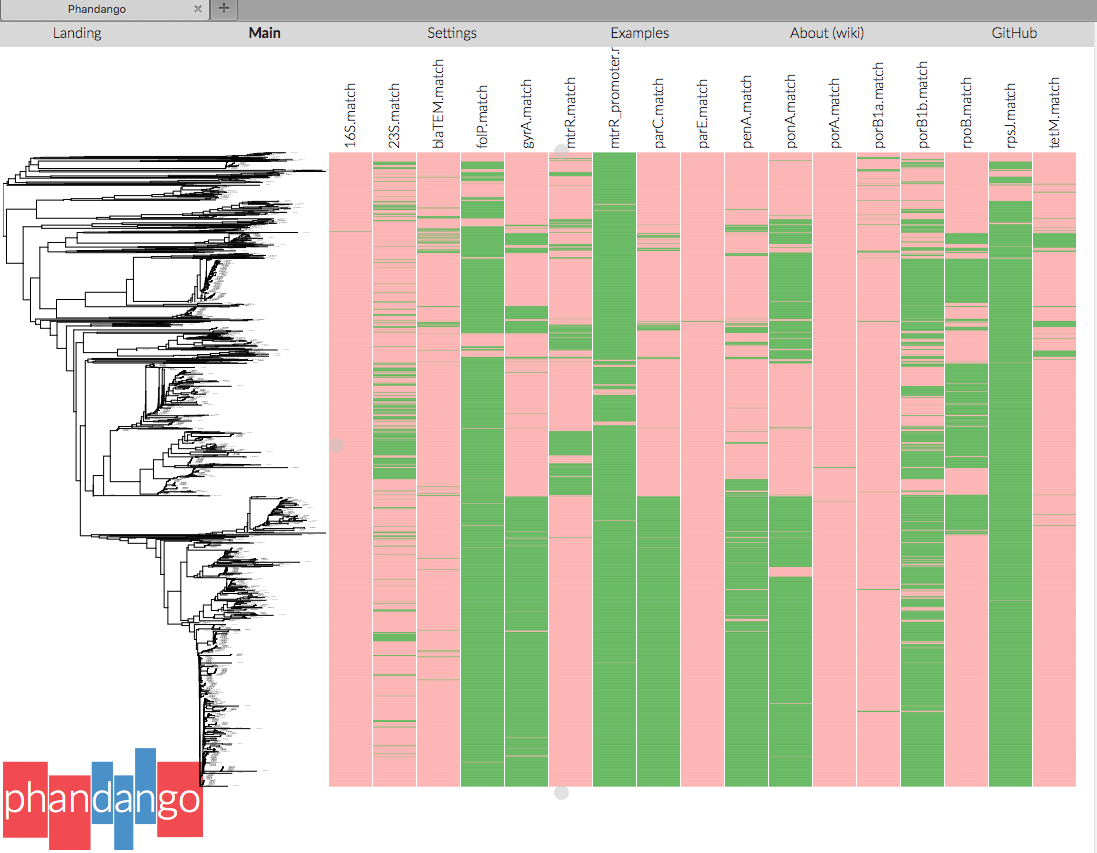
\includegraphics{Screenshots/screenshot.phandango.default.png}
\caption{Default Layout}
\end{figure}


\newpage




    This a very high-level summary of the data. For each cluster, it is
simply saying whether or not each sample has a `match'. Green means a
match, and pink means not a match. For presence/absence genes, this
means that the gene must simply be there to count as a match. If it is a
``variant only'' gene, then the gene must be there and one of the
variants that we told ARIBA about earlier when
\href{make_custom_db.ipynb}{generating the ARIBA database}.

    \hypertarget{more-information-per-cluster}{%
\subsection{More information per
cluster}\label{more-information-per-cluster}}

In addition to a simple ``yes'' or ``no'' as to whether a sample
``matches'' a given cluster (as explained above), more columns can be
output for each cluster. See the
\href{https://github.com/sanger-pathogens/ariba/wiki/Task:-summary}{ARIBA
summary wiki page} for a full description of the options.

Adding more columns can result in a very wide plot, so we will just look
at 23S from now on, using the option \texttt{-\/-only\_clusters\ 23S}.
Adding the option \texttt{-\/-preset\ all} will show all available
columns for the 23S cluster:

\begin{terminalinput}
\begin{Verbatim}[commandchars=\\\{\}]
\llap{\color{black}\LARGE\faKeyboardO\hspace{1em}} ariba summary \PYZhy{}\PYZhy{}only\PYZus{}clusters 23S \PYZhy{}\PYZhy{}preset cluster\PYZus{}all \PYZhy{}\PYZhy{}no\PYZus{}tree \PY{l+s+se}{\PYZbs{}}
          \PYZhy{}\PYZhy{}fofn data/filenames.fofn out data/ARIBA\PYZus{}reports/*.tsv
\end{Verbatim}
\end{terminalinput}

    As before, drag and drop the files \texttt{out.phandango.csv} and
\texttt{data/tree\_for\_phandango.tre} into the window. This time the
result should look like this:

    \begin{figure}[H]
\centering
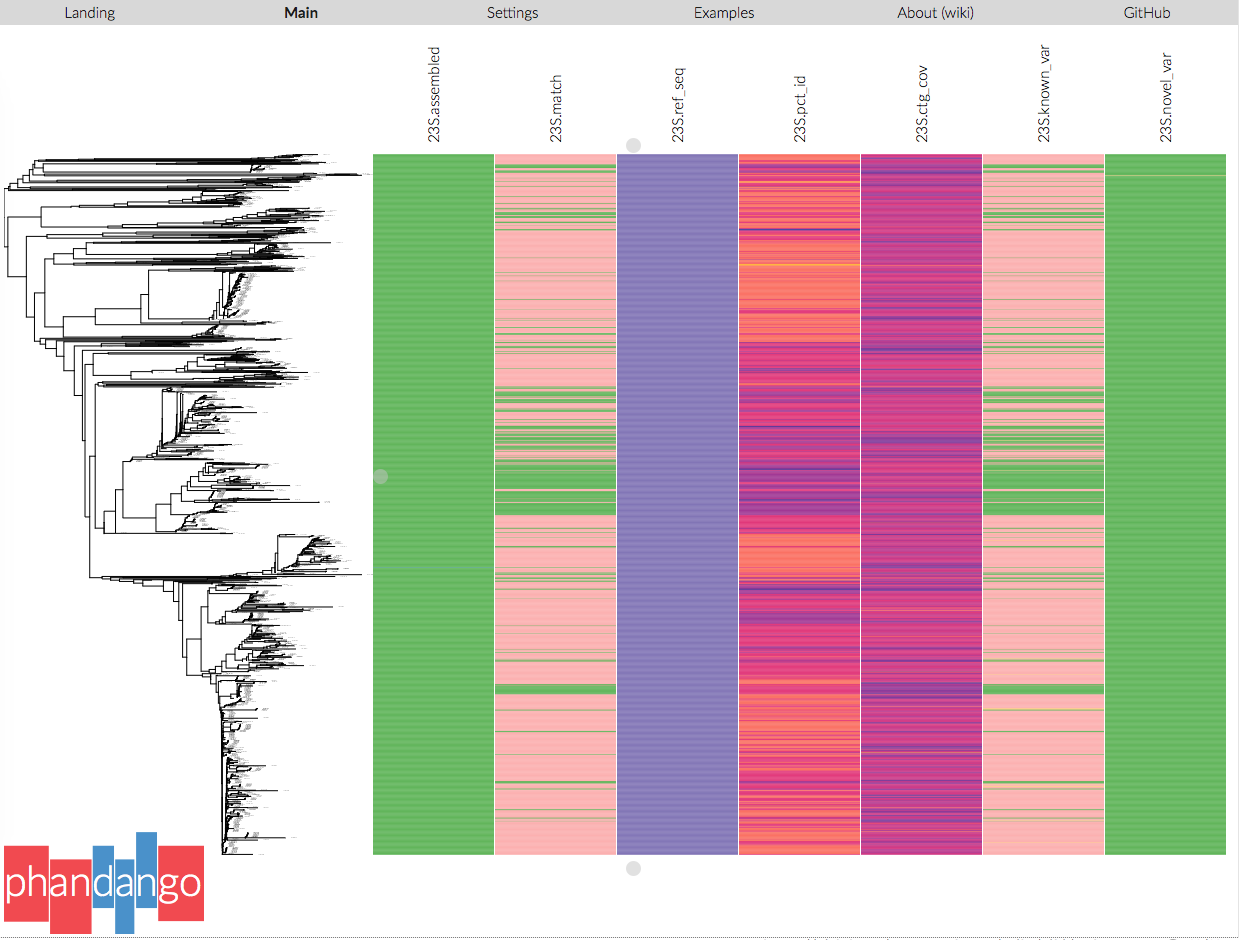
\includegraphics{Screenshots/screenshot.phandango.23S.cluster_all.png}
\caption{Phandango 23S cluster\_all}
\end{figure}

    Now there are seven columns, showing various findings from ARIBA for
23S. These columns are described in the
\href{https://github.com/sanger-pathogens/ariba/wiki/Task:-summary}{ARIBA
summary wiki page}.

You can control exactly which of the seven cluster columns are output
using the option \texttt{-\/-cluster\_cols} instead of
\texttt{-\/-preset}. For example, this will show just the ``match'' and
``pct\_id'' columns:

\begin{terminalinput}
\begin{Verbatim}[commandchars=\\\{\}]
\llap{\color{black}\LARGE\faKeyboardO\hspace{1em}} ariba summary \PYZhy{}\PYZhy{}only\PYZus{}clusters 23S \PYZhy{}\PYZhy{}cluster\PYZus{}cols match,pct\PYZus{}id \PY{l+s+se}{\PYZbs{}}
            \PYZhy{}\PYZhy{}no\PYZus{}tree \PYZhy{}\PYZhy{}fofn data/filenames.fofn out \PY{l+s+se}{\PYZbs{}}
            data/ARIBA\PYZus{}reports/*.tsv
\end{Verbatim}
\end{terminalinput}

    \hypertarget{variants}{%
\subsection{Variants}\label{variants}}

In the previous screenshot, where the option
\texttt{-\/-preset\ cluster\_all}, there are two variant columns:
``known\_var'' and ``novel\_var''. Green means ``yes'' and pink means
``no''. Here, we are considering a variant to be a difference bewteen
the reference sequence and the assembly contig from the reads. The
known\_var column indicates whether each sample has any variant that is
known to ARIBA, which means it was included when the original ARIBA
database was generated. The novel\_var column indicates whether or not a
sample has any variant that is not already known to ARIBA.

We can view the calls for all the known variants by adding the
\texttt{-\/-known\_variants} option:

\begin{terminalinput}
\begin{Verbatim}[commandchars=\\\{\}]
\llap{\color{black}\LARGE\faKeyboardO\hspace{1em}} ariba summary \PYZhy{}\PYZhy{}only\PYZus{}clusters 23S \PYZhy{}\PYZhy{}known\PYZus{}variants \PYZhy{}\PYZhy{}no\PYZus{}tree \PY{l+s+se}{\PYZbs{}}
          \PYZhy{}\PYZhy{}fofn data/filenames.fofn out data/ARIBA\PYZus{}reports/*.tsv
\end{Verbatim}
\end{terminalinput}

    As before, drag and drop the files \texttt{out.phandango.csv} and
\texttt{data/tree\_for\_phandango.tre} into the window. This time the
result should like this:

    \begin{figure}[H]
\centering
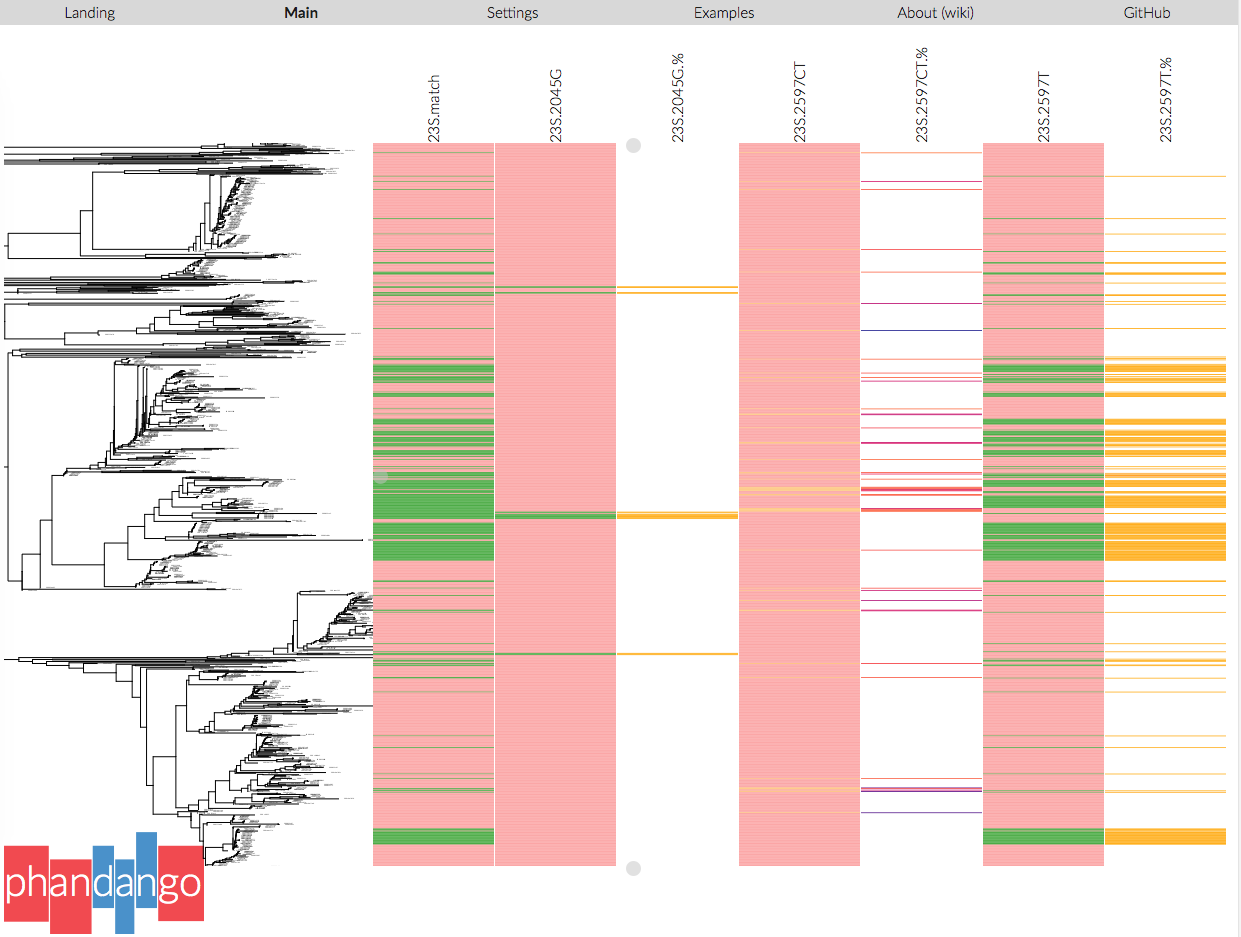
\includegraphics{Screenshots/screenshot.phandango.23S.known_vars.png}
\caption{Phandango 23S known\_variants}
\end{figure}

    Each known SNP and whether or not it is present is shown, but you may
have noticed there are three colours. Green means ``yes'', orange means
``heterozygous'', and pink means ``no''. \textit{N. gonorrhoeae} has four
copies of 23S. A SNP could be present in none, some, or all copies.
Where it is present in 1,2, or 3 copies, it is called ``heterozygous''
by ARIBA. Consider the SNP 2597CT in column 4, and column 5 to the right
``2597CT.\%''. Samples either do not have this SNP, or have heterozygous
calls. The 2597CT.\% shows the percent of reads that have the SNP, when
mapped to the contig. Hover over the coloured blocks in Phandango to see
the percentage.

\begin{terminalinput}
\begin{Verbatim}[commandchars=\\\{\}]
\llap{\color{black}\LARGE\faKeyboardO\hspace{1em}} ariba summary \PYZhy{}\PYZhy{}only\PYZus{}clusters 23S \PYZhy{}\PYZhy{}novel\PYZus{}variants \PYZhy{}\PYZhy{}no\PYZus{}tree \PY{l+s+se}{\PYZbs{}}
          \PYZhy{}\PYZhy{}fofn data/filenames.fofn out data/ARIBA\PYZus{}reports/*.tsv
\end{Verbatim}
\end{terminalinput}

    Now Phandango shows all variants found in any of the samples (even if
the variant is unique to one sample). This results in a lot of columns!

    \begin{figure}[H]
\centering
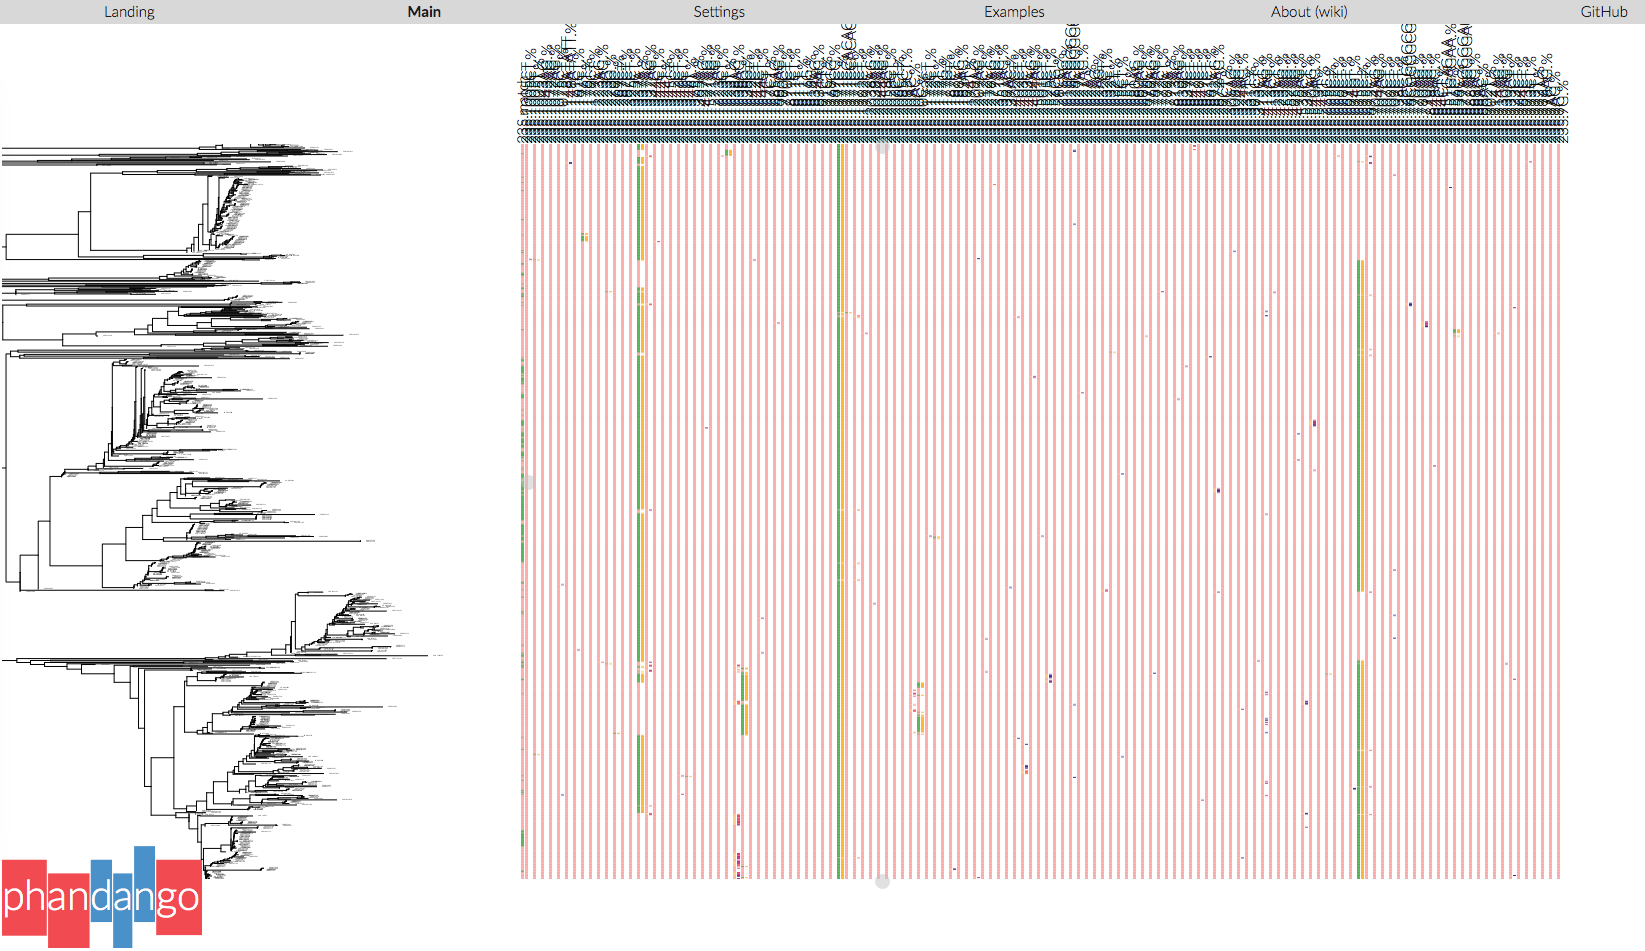
\includegraphics{Screenshots/screenshot.phandango.23S.novel_vars.png}
\caption{Phandango 23S novel\_variants}
\end{figure}

    Now go to the next part of the tutorial where we
\href{micplot.ipynb}{Investigate MIC data in relation to variants in the
samples}.

You can also \href{index.ipynb}{return to the index} or revisit the
\href{phandango.ipynb}{previous section}.


    % Add a bibliography block to the postdoc



\newpage





    \hypertarget{investigating-mic-data}{%
\section{Investigating MIC data}\label{investigating-mic-data}}

We will use the \textit{N. gonorrhoeae} dataset. This tutorial includes
pre-computed output of running ARIBA on all the samples, and the ARIBA
database that was made in the \href{make_custom_db.ipynb}{first
section}. Do not worry if you did not follow that part of the tutorial -
we will use a pre-computed version of the database called
\texttt{data/Ref/Ngo\_ARIBAdb/}.

ARIBA has a function called ``micplot'' that generates plots showing the
distribution of MICs across samples with different combinations of
genotypes. To use it, a file is required of MIC data for each sample and
at least one drug. It looks like this:

\begin{terminalinput}
\begin{Verbatim}[commandchars=\\\{\}]
\llap{\color{black}\LARGE\faKeyboardO\hspace{1em}} head data/mic\PYZus{}data.tsv
\end{Verbatim}
\end{terminalinput}

    The first column must be named ``Sample'' and have names that exactly
match those in ARIBA summary files used as input to micplot (we will see
this shortly). The remaining columns should contain drug names and MIC
scores, however, note that the first two columns contain other data that
will be ignored by ARIBA. When ARIBA loads the file, it tries to convert
everything in columns 2 onwards to numbers and assign a value of ``NA''
when this is not possible.

To run micplot, we need an MIC file, like the one above, and an ARIBA
summary file (as described in the \href{phandango.ipynb}{previous
section}). This generates a summary of known 23S and mtrR mutations and
includes the ``assembled'' cluster column, so that interrupted mtrR can
be identified:

\begin{terminalinput}
\begin{Verbatim}[commandchars=\\\{\}]
\llap{\color{black}\LARGE\faKeyboardO\hspace{1em}} ariba summary \PYZhy{}\PYZhy{}row\PYZus{}filter n \PYZhy{}\PYZhy{}cluster\PYZus{}cols assembled,known\PYZus{}var \PY{l+s+se}{\PYZbs{}}
            \PYZhy{}\PYZhy{}only\PYZus{}clusters 23S,mtrR \PYZhy{}\PYZhy{}v\PYZus{}groups \PYZhy{}\PYZhy{}no\PYZus{}tree \PY{l+s+se}{\PYZbs{}}
            \PYZhy{}\PYZhy{}fofn data/filenames.fofn summary.AZMknowngroups
\end{Verbatim}
\end{terminalinput}

    Now we can run micplot using the new file
\texttt{summary.AZMknowngroups.csv} and the MIC file
\texttt{data/mic\_data.tsv}, showing the MIC data for azithromicin
compared with the different combinations of sequences and known
mutations in 23S and mtrR:

\begin{terminalinput}
\begin{Verbatim}[commandchars=\\\{\}]
\llap{\color{black}\LARGE\faKeyboardO\hspace{1em}} ariba micplot data/Ref/Ngo\PYZus{}ARIBAdb/ \PYZhy{}\PYZhy{}interrupted Azithromycin \PY{l+s+se}{\PYZbs{}}
            data/mic\PYZus{}data.tsv summary.AZMknowngroups.csv \PY{l+s+se}{\PYZbs{}}
            micplot.AZMknowngroups
\end{Verbatim}
\end{terminalinput}

    This produced a pdf file \texttt{micplot.AZMknowngroups.pdf} that looks
like this:

    \begin{figure}[H]
\centering
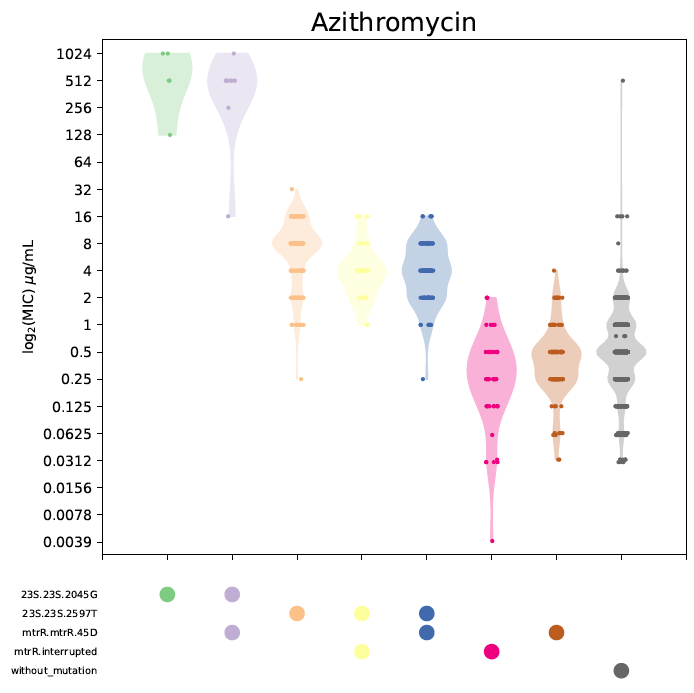
\includegraphics{Screenshots/screenshot.micplot.AZMknowngroups.png}
\caption{micplot AZMknowngroups}
\end{figure}

    There are various options that can be changed. We will show some of them
here, but try running \texttt{ariba\ micplot\ -\/-help} to see all the
options.

\hypertarget{horizontal-lines}{%
\subsection{Horizontal lines}\label{horizontal-lines}}

Horizontal lines can be added to indicate import cutoffs for MIC data,
in this case 0.25 and 2, using the option \texttt{-\/-hlines}.

\begin{terminalinput}
\begin{Verbatim}[commandchars=\\\{\}]
\llap{\color{black}\LARGE\faKeyboardO\hspace{1em}} ariba micplot data/Ref/Ngo\PYZus{}ARIBAdb/ \PYZhy{}\PYZhy{}interrupted \PYZhy{}\PYZhy{}hlines 0.25,2 \PY{l+s+se}{\PYZbs{}}
            Azithromycin data/mic\PYZus{}data.tsv summary.AZMknowngroups.csv \PY{l+s+se}{\PYZbs{}}
            micplot.AZMknowngroups
\end{Verbatim}
\end{terminalinput}



\newpage



    Here is the result:

    \begin{figure}[H]
\centering
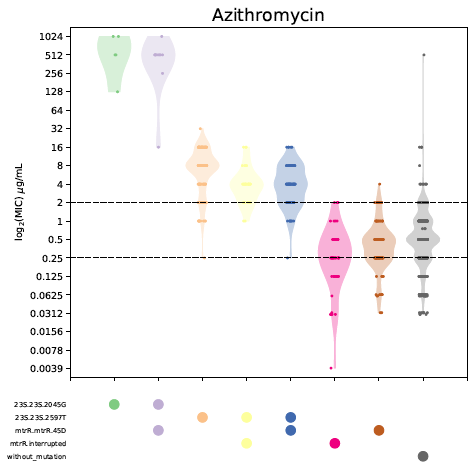
\includegraphics{Screenshots/screenshot.micplot.AZMknowngroups.hlines.png}
\caption{micplot hlines}
\end{figure}

    \hypertarget{plot-styles}{%
\subsection{Plot styles}\label{plot-styles}}

In the plots above, there is one point per sample. It can be hard to see
how many points there are, despite there being jittering applied to the
horizontal position. We can change the style to group the points
together and plot circles of sizes proportional to the number of
samples, using the option \texttt{-\/-point\_size}. This option
determines the size of the points, but when set to zero if groups the
points together.

\begin{terminalinput}
\begin{Verbatim}[commandchars=\\\{\}]
\llap{\color{black}\LARGE\faKeyboardO\hspace{1em}} ariba micplot data/Ref/Ngo\PYZus{}ARIBAdb/ \PYZhy{}\PYZhy{}interrupted \PYZhy{}\PYZhy{}hlines 0.25,2 \PY{l+s+se}{\PYZbs{}}
            \PYZhy{}\PYZhy{}point\PYZus{}size \PY{l+m}{0} Azithromycin data/mic\PYZus{}data.tsv \PY{l+s+se}{\PYZbs{}}
            summary.AZMknowngroups.csv micplot.AZMknowngroups
\end{Verbatim}
\end{terminalinput}


\newpage


    Here is the result:

    \begin{figure}[H]
\centering
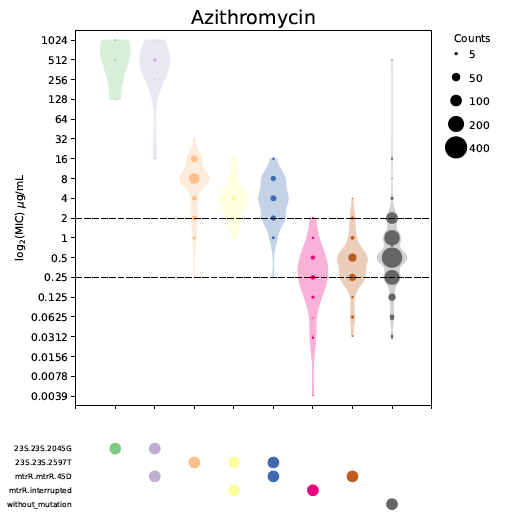
\includegraphics{Screenshots/screenshot.micplot.AZMknowngroups.point_zero.png}
\caption{micplot point size zero}
\end{figure}

    You can choose to not show the violin plots or the dots in the upper
plot, using the option \texttt{-\/-plot\_types}. The default is
\texttt{violin,point}, which means show both. To only show the dots:

\begin{terminalinput}
\begin{Verbatim}[commandchars=\\\{\}]
\llap{\color{black}\LARGE\faKeyboardO\hspace{1em}} ariba micplot data/Ref/Ngo\PYZus{}ARIBAdb/ \PYZhy{}\PYZhy{}interrupted \PYZhy{}\PYZhy{}hlines 0.25,2 \PY{l+s+se}{\PYZbs{}}
         \PYZhy{}\PYZhy{}plot\PYZus{}types point \PYZhy{}\PYZhy{}point\PYZus{}size \PY{l+m}{0} \PY{l+s+se}{\PYZbs{}}
         Azithromycin data/mic\PYZus{}data.tsv summary.AZMknowngroups.csv \PY{l+s+se}{\PYZbs{}}
         micplot.AZMknowngroups
\end{Verbatim}
\end{terminalinput}



\newpage



    Here is the result:

    \begin{figure}[H]
\centering
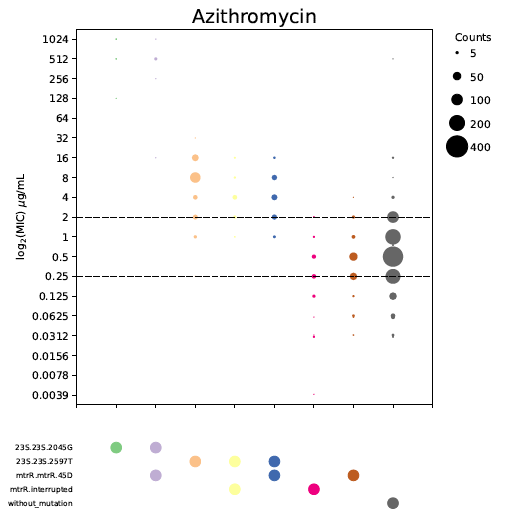
\includegraphics{Screenshots/screenshot.micplot.AZMknowngroups.dots_only.png}
\caption{micplot dots only}
\end{figure}

    \hypertarget{colours}{%
\subsection{Colours}\label{colours}}

There are various colour options - see the
\href{http://matplotlib.org/users/colormaps.html}{matplotlib colourmaps
page} for all of the available colour palettes. The default is
``Accent'', which has 8 colours. ARIBA will cycle through these,
repeating colours if there are more than 8 columns in the plot. The
palette can be changed using the option \texttt{-\/-colourmap}.

\begin{terminalinput}
\begin{Verbatim}[commandchars=\\\{\}]
\llap{\color{black}\LARGE\faKeyboardO\hspace{1em}} ariba micplot data/Ref/Ngo\PYZus{}ARIBAdb/ \PYZhy{}\PYZhy{}interrupted \PYZhy{}\PYZhy{}hlines 0.25,2 \PY{l+s+se}{\PYZbs{}}
         \PYZhy{}\PYZhy{}colourmap PiYG \PYZhy{}\PYZhy{}point\PYZus{}size \PY{l+m}{0} Azithromycin data/mic\PYZus{}data.tsv \PY{l+s+se}{\PYZbs{}}
         summary.AZMknowngroups.csv micplot.AZMknowngroups
\end{Verbatim}
\end{terminalinput}



\newpage



    Here is the result:

    \begin{figure}[H]
\centering
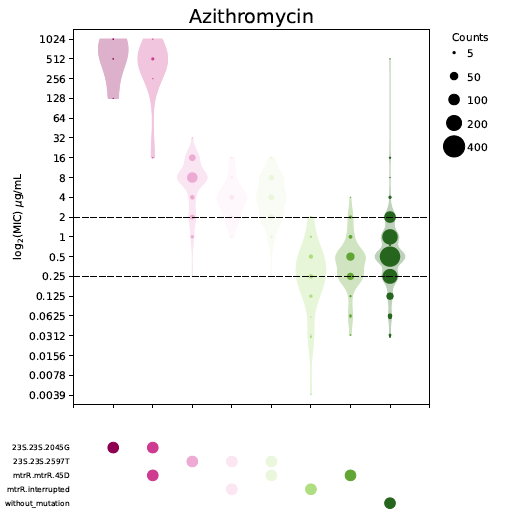
\includegraphics{Screenshots/screenshot.micplot.AZMknowngroups.PiYG.png}
\caption{micplot PiYG}
\end{figure}

    The palette PiYG is continuous, and is almost white in the middle. This
is not ideal. We can skip the range in the middle, specifically 40-60\%,
using the option \texttt{-\/-colour\_skip}:

\begin{terminalinput}
\begin{Verbatim}[commandchars=\\\{\}]
\llap{\color{black}\LARGE\faKeyboardO\hspace{1em}} ariba micplot data/Ref/Ngo\PYZus{}ARIBAdb/ \PYZhy{}\PYZhy{}interrupted \PYZhy{}\PYZhy{}hlines 0.25,2 \PY{l+s+se}{\PYZbs{}}
         \PYZhy{}\PYZhy{}colourmap PiYG \PYZhy{}\PYZhy{}colour\PYZus{}skip 0.35,0.65 \PYZhy{}\PYZhy{}point\PYZus{}size \PY{l+m}{0} \PY{l+s+se}{\PYZbs{}}
         Azithromycin data/mic\PYZus{}data.tsv summary.AZMknowngroups.csv \PY{l+s+se}{\PYZbs{}}
         micplot.AZMknowngroups
\end{Verbatim}
\end{terminalinput}



\newpage



    Here is the new plot:

    \begin{figure}[H]
\centering
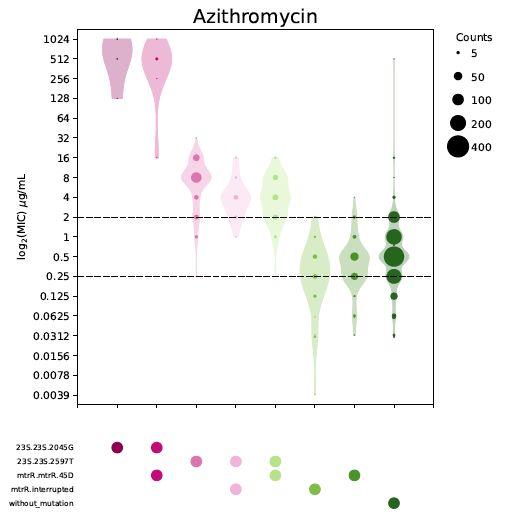
\includegraphics{Screenshots/screenshot.micplot.AZMknowngroups.colour_skip.png}
\caption{micplot colour\_skip}
\end{figure}

    The number of colours can be set to less than the number of columns
using the option \texttt{-\/-number\_of\_colours}. This makes ARIBA
cycle the colours. Here is an example using the first three colours from
the ``Dark2'' colour palette:

\begin{terminalinput}
\begin{Verbatim}[commandchars=\\\{\}]
\llap{\color{black}\LARGE\faKeyboardO\hspace{1em}} ariba micplot data/Ref/Ngo\PYZus{}ARIBAdb/ \PYZhy{}\PYZhy{}interrupted \PYZhy{}\PYZhy{}hlines 0.25,2 \PY{l+s+se}{\PYZbs{}}
         \PYZhy{}\PYZhy{}colourmap Dark2 \PYZhy{}\PYZhy{}number\PYZus{}of\PYZus{}colours \PY{l+m}{3} \PYZhy{}\PYZhy{}point\PYZus{}size \PY{l+m}{0} \PY{l+s+se}{\PYZbs{}}
         Azithromycin data/mic\PYZus{}data.tsv summary.AZMknowngroups.csv \PY{l+s+se}{\PYZbs{}}
         micplot.AZMknowngroups
\end{Verbatim}
\end{terminalinput}


\newpage


    And we only have three colours:

    \begin{figure}[H]
\centering
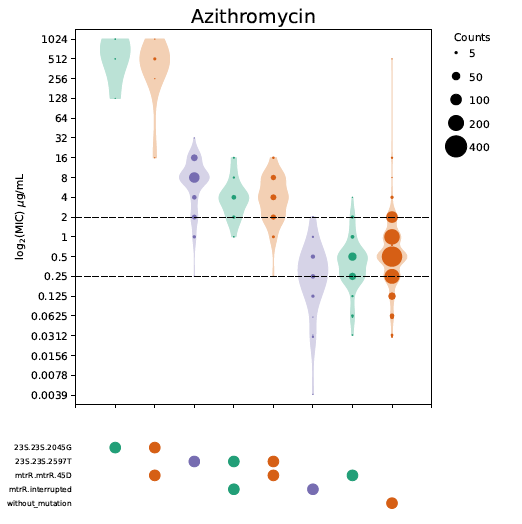
\includegraphics{Screenshots/screenshot.micplot.AZMknowngroups.3colours.png}
\caption{micplot 3 colours}
\end{figure}

    Setting the number of colours to one results in a black and white
figure.

\begin{terminalinput}
\begin{Verbatim}[commandchars=\\\{\}]
\llap{\color{black}\LARGE\faKeyboardO\hspace{1em}} ariba micplot data/Ref/Ngo\PYZus{}ARIBAdb/ \PYZhy{}\PYZhy{}interrupted \PYZhy{}\PYZhy{}hlines 0.25,2 \PY{l+s+se}{\PYZbs{}}
         \PYZhy{}\PYZhy{}number\PYZus{}of\PYZus{}colours \PY{l+m}{1} \PYZhy{}\PYZhy{}point\PYZus{}size \PY{l+m}{0} Azithromycin \PY{l+s+se}{\PYZbs{}}
         data/mic\PYZus{}data.tsv summary.AZMknowngroups.csv micplot.AZMknowngroups
\end{Verbatim}
\end{terminalinput}



\newpage


    Here is the black and white figure:

    \begin{figure}[H]
\centering
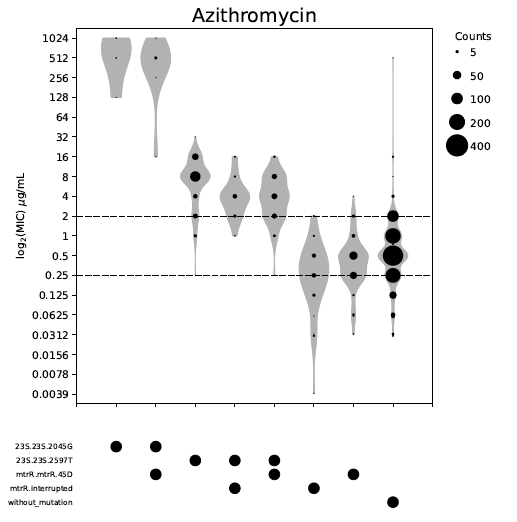
\includegraphics{Screenshots/screenshot.micplot.AZMknowngroups.blackwhite.png}
\caption{micplot black and white}
\end{figure}

    This is the end of the tutorial. You can \href{index.ipynb}{return to
the index} or revisit the \href{phandango.ipynb}{previous section}.


    % Add a bibliography block to the postdoc



\end{document}
